\textbf{(1)} O fluoreto de nitrila (\ce{NO2F}) é um gás incolor e um agente oxidante forte empregado como agente fluoretante. É uma espécie molecular (não iônica) e possui estrutura planar. O estudo de suas propriedades termodinâmicas e de sua formação foi realizado em 1962 por E. Tschuikow-Row\textsuperscript{1}, o qual verificou o mecanismo de formação e sua dependência com a temperatura através de espectroscopias vibracionais (Raman e IV).\\

A reação global observada foi:

\begin{align*}
    2\,\ce{NO2}(g) + \ce{F2}(g) \rightarrow 2\,\ce{NO2F}(g)
\end{align*}

 Essa reação, no entanto, apresentou um mecanismo complexo cuja lei de velocidade é dada por:

\begin{align*}
    v = k[\ce{NO2}][\ce{F2}]
\end{align*}

e o estudo de suas propriedades termodinâmicas apresentou variação da constante de equilíbrio ($K_{\text{eq}}$) em função da temperatura na etapa determinante (etapa lenta), conforme (ln$K_{\text{eq}}$) na tabela abaixo:

\begin{center}
\begin{tabular}{|c|c|c|c|c|c|c|c|c|c|}
\hline
\textbf{T / K} & 200 & 300 & 400 & 500 & 600 & 700 & 800 & 900 & 1000 \\
\hline
\textbf{ln $K_{\text{eq}}$} & 7,55 & 14,43 & 17,84 & 19,85 & 21,16 & 22,08 & 22,72 & 23,28 & 23,67 \\
\hline
\end{tabular}
\end{center}

\bigskip

Com todas essas informações em mãos:\\

\textbf{a)} Proponha o mecanismo de reação para a formação do \ce{NO2F} e explicite a etapa determinante;\\

\textbf{Resposta:} 

Para propor o mecanismo de reação para a formação do \ce{NO2F}, partimos da equação global observada:
\begin{align*}
2\ \ce{NO2}(g) + \ce{F2}(g) \rightarrow 2\ \ce{NO2F}(g)
\end{align*}

Embora a reação pareça simples, estudos experimentais revelaram que ela ocorre por um mecanismo mais complexo, sendo a sua velocidade regida pela expressão:
\begin{align*}
v = k[\ce{NO2}][\ce{F2}]
\end{align*}

Essa lei de velocidade indica que a etapa determinante (ou etapa lenta) do processo envolve uma colisão entre uma molécula de \ce{NO2} e uma molécula de \ce{F2}, ou seja, é uma etapa bimolecular. A partir disso, propõe-se o seguinte mecanismo:

\textit{Etapa lenta (determinante):}
\begin{align*}
\ce{NO2 + F2 <=> [NO2 \cdots F2]^{\ddagger}}
\end{align*}

Nesta etapa, as moléculas colidem e formam um complexo ativado de alta energia, sendo essa a etapa que controla a velocidade global da reação.

\textit{Etapa rápida subsequente:}
\begin{align*}
\ce{[NO2 \cdots F2]^{\ddagger} -> NO2F + F}
\end{align*}

Aqui ocorre a quebra da ligação F–F e formação de uma nova ligação N–F, liberando um radical flúor.

\textit{Etapa final:}
\begin{align*}
\ce{F + NO2 -> NO2F}
\end{align*}

O radical flúor gerado na etapa anterior rapidamente reage com uma nova molécula de \ce{NO2} para formar mais uma molécula de \ce{NO2F}, completando a reação global.

\begin{align*}
&\ce{NO2 + F2 <=> [NO2 \cdots F2]^{\ddagger}} \hspace{1.0cm} \text{(etapa lenta)}\\
&\ce{[NO2 \cdots F2]^{\ddagger} -> NO2F + F} \hspace{0.9cm} \text{(etapa rápida)}\\
&\ce{F + NO2 -> NO2F} \hspace{2.2cm} \text{(etapa final)}\\
\midrule %Alguém sabe ajeitar essa linha maldita?
&\ce{2NO2 + F2 -> 2NO2F} \hspace{1.6cm} \text{(equação global)}
\end{align*}

Dessa forma, o mecanismo é consistente tanto com a estequiometria global quanto com a lei de velocidade observada experimentalmente, e evidencia que a etapa determinante é a formação do intermediário a partir de \ce{NO2} e \ce{F2}.

\vspace{0.4cm}

\textbf{b)} Proponha a estrutura do complexo ativado para essa reação bimolecular;\\

\textbf{Resposta:} 

Para representar a estrutura do complexo ativado dessa reação bimolecular, é necessário considerar que, durante a colisão entre \ce{NO2} e \ce{F2}, ocorre uma reorganização eletrônica na qual uma das ligações F–F começa a se romper ao mesmo tempo que uma nova ligação N–F começa a se formar. Esse estado de transição pode ser representado por uma estrutura em que os átomos ainda não estão completamente ligados, caracterizando o chamado “complexo ativado” ou “estado de transição”.

A estrutura pode ser descrita como:
\begin{align*}
\ce{[NO2 \cdots F-F]^{\ddagger}}
\end{align*}

Nesse intermediário, o flúor mais próximo do nitrogênio do \ce{NO2} apresenta uma ligação parcialmente formada com o N, enquanto a ligação F–F encontra-se parcialmente rompida. Além disso, a geometria ao redor do nitrogênio provavelmente se torna levemente distorcida em relação ao plano original da molécula, dada a reorganização eletrônica em curso. Essa estrutura representa o ponto de maior energia no caminho da reação, ou seja, o topo da barreira energética que os reagentes devem superar para formar os produtos.

\vspace{0.4cm}

\textbf{c)} Apresente a curva de energia potencial de formação do \ce{NO2F}, apontando a região da curva onde ocorre a formação do complexo ativado. De acordo com suas observações, essa reação é endotérmica ou exotérmica? Explique com o devido formalismo.\\

\textbf{Resposta:} 

Com base nos dados fornecidos sobre a constante de equilíbrio (\(K_\text{eq}\)) da etapa determinante em diferentes temperaturas, é possível analisar a natureza energética do processo. A tabela mostra que o valor de \(\ln(K_\text{eq})\) aumenta com o aumento da temperatura, o que implica que a constante de equilíbrio também cresce. Isso pode ser interpretado por meio da equação de Van’t Hoff:
\begin{align*}
\ln K = -\frac{\Delta H^\circ}{R} \cdot \frac{1}{T} + \frac{\Delta S^\circ}{R}
\end{align*}

Segundo essa equação, se \(\ln(K)\) aumenta com a elevação da temperatura, isso indica que \(\Delta H^\circ\) é positivo, pois somente assim o termo \(-\frac{\Delta H^\circ}{R} \cdot \frac{1}{T}\) se torna menos negativo à medida que \(T\) cresce. Isso significa que a etapa determinante do mecanismo é endotérmica, ou seja, consome energia do meio para ocorrer.

Essa análise foi representada pelo diagrama de energia potencial em função da coordenada de reação (\cref{diagrama}). Nesse gráfico, os reagentes se encontram em um patamar energético inicial. À medida que a reação prossegue, a energia do sistema aumenta até atingir um máximo, correspondente ao complexo ativado — o ponto mais instável e de maior energia do processo. Após ultrapassada essa barreira, a energia diminui com a formação dos produtos.

    \begin{figure}[H]
        \centering
        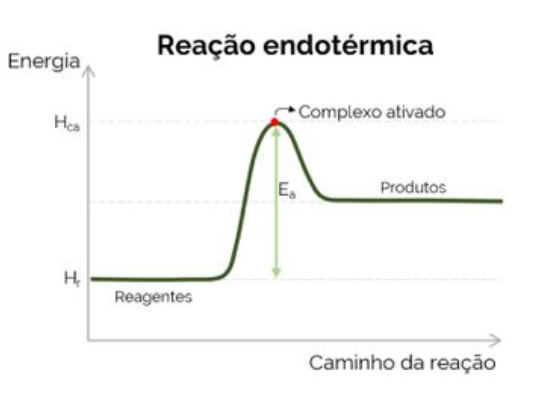
\includegraphics[width=0.35\linewidth]{fig/grafico.png}
        \caption{curva de energia potencial de formação do \ce{NO2F}}
        \label{diagrama}
    \end{figure}

Como a energia dos produtos é maior do que a dos reagentes, a variação de entalpia total da reação (\(\Delta H\)) é positiva, reforçando que o processo é endotérmico. A energia de ativação (\(E_\text{a}\)) corresponde à diferença entre os reagentes e o complexo ativado, e sua magnitude está relacionada à taxa com que a reação ocorre: quanto maior a \(E_\text{a}\), mais lenta é a reação, justificando a sua presença como etapa determinante.

Portanto, a partir dos dados fornecidos e da análise do gráfico de energia, conclui-se que a formação do \ce{NO2F} apresenta uma etapa lenta que é endotérmica, com formação de um complexo ativado de alta energia, e que a reação global ocorre mediante superação dessa barreira, em consonância com o modelo energético das reações químicas e o formalismo termodinâmico.
